\documentclass[tikz,border=10pt,multi=tikzpicture]{standalone}
\usepackage{amsmath}
\usepackage{xcolor}
\usetikzlibrary{calc}
\definecolor{mainblue}{HTML}{001158}
\definecolor{accent}{HTML}{8592bc}
\definecolor{lightaccent}{HTML}{e7e9f2}
\definecolor{lasercolor}{HTML}{e63946}
\definecolor{damagecolor}{HTML}{e76f51}
\definecolor{wavecolor}{HTML}{2a9d8f}

\tikzset{
  rootnode/.style={rectangle, rounded corners=4pt, draw=mainblue, fill=mainblue, text=white, minimum width=6.2cm, minimum height=1.0cm, font=\bfseries\large, align=center},
  pillarnode/.style={rectangle, rounded corners=4pt, draw=mainblue, fill=accent, text=white, minimum width=5.0cm, minimum height=1.0cm, font=\bfseries, align=center},
  leafnode/.style={rectangle, rounded corners=3pt, draw=mainblue, fill=lightaccent, text=mainblue, minimum width=4.6cm, minimum height=0.9cm, font=\small, align=center},
  edge/.style={mainblue, line width=1.1pt}
}

\begin{document}

% ---------- PAGE 1: two research pillars (tree) ----------
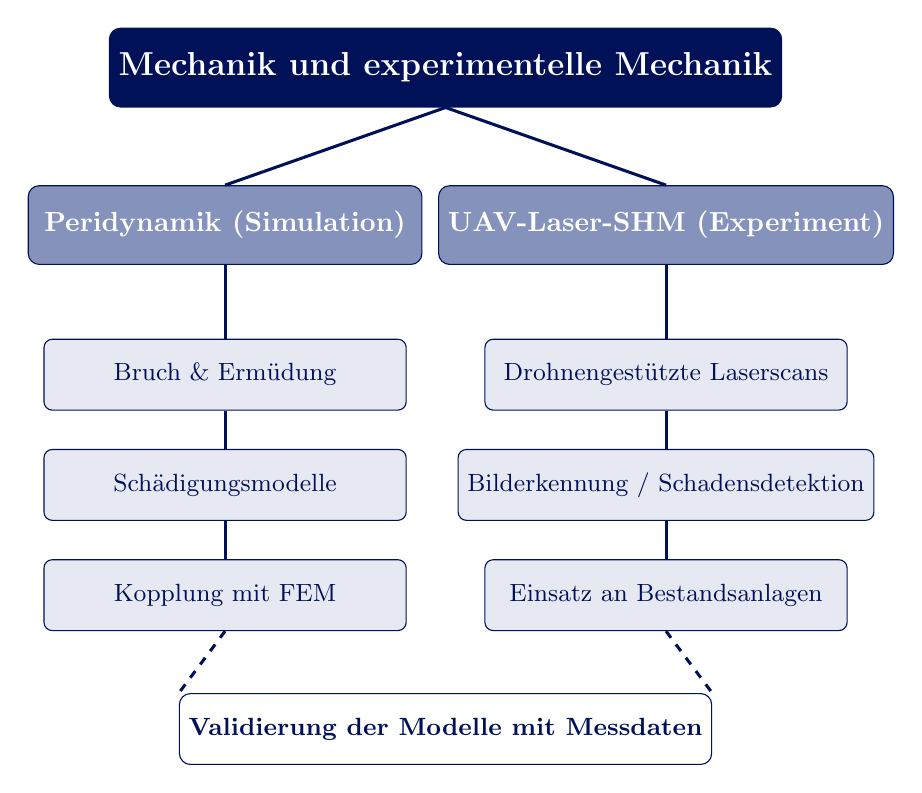
\begin{tikzpicture}[>=stealth]
  \node[rootnode] (root) at (5.0,8.6) {Mechanik und experimentelle Mechanik};

  \node[pillarnode] (pd) at (2.2,6.6) {Peridynamik (Simulation)};
  \node[pillarnode] (shm) at (7.8,6.6) {UAV-Laser-SHM (Experiment)};

  \draw[edge] (root.south) -- (pd.north);
  \draw[edge] (root.south) -- (shm.north);

  \node[leafnode] (pd1) at (2.2,4.7) {Bruch \& Ermüdung};
  \node[leafnode] (pd2) at (2.2,3.3) {Schädigungsmodelle};
  \node[leafnode] (pd3) at (2.2,1.9) {Kopplung mit FEM};

  \draw[edge] (pd.south) -- (pd1.north);
  \draw[edge] (pd1.south) -- (pd2.north);
  \draw[edge] (pd2.south) -- (pd3.north);

  \node[leafnode] (shm1) at (7.8,4.7) {Drohnengestützte Laserscans};
  \node[leafnode] (shm2) at (7.8,3.3) {Bilderkennung / Schadensdetektion};
  \node[leafnode] (shm3) at (7.8,1.9) {Einsatz an Bestandsanlagen};

  \draw[edge] (shm.south) -- (shm1.north);
  \draw[edge] (shm1.south) -- (shm2.north);
  \draw[edge] (shm2.south) -- (shm3.north);

  % synergy connector
  \node[rectangle, rounded corners=4pt, draw=mainblue, fill=white, text=mainblue, minimum width=6.6cm, minimum height=0.9cm, font=\bfseries\small, align=center] (synergy) at (5.0,0.2) {Validierung der Modelle mit Messdaten};
  \draw[edge, dashed] (pd3.south) -- (synergy.north west);
  \draw[edge, dashed] (shm3.south) -- (synergy.north east);
\end{tikzpicture}

% ---------- PAGE 2: drone-laser SHM concept / pipeline ----------
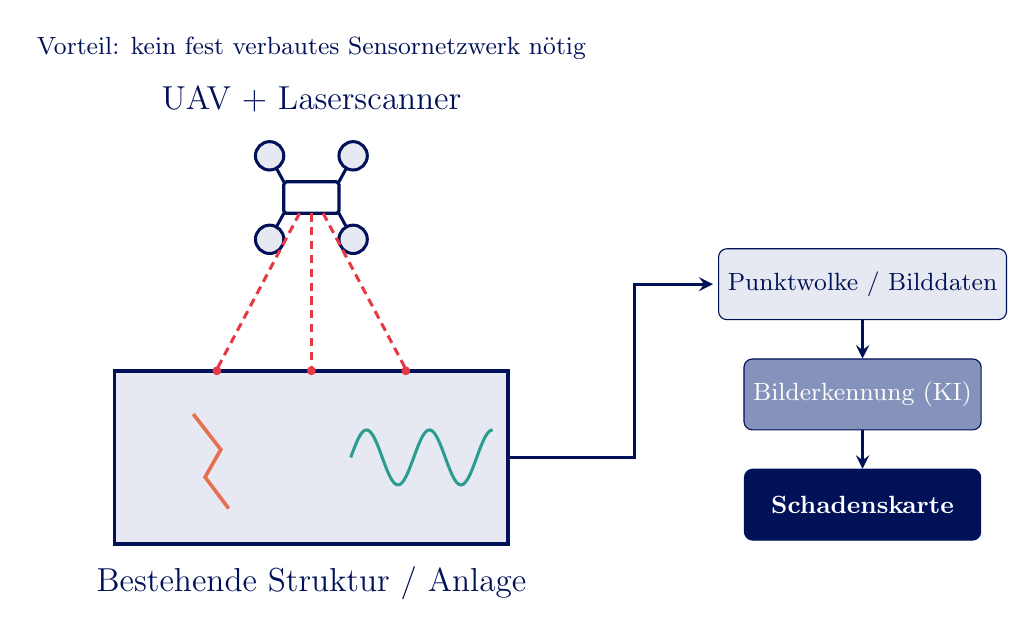
\begin{tikzpicture}[>=stealth, font=\large]
  % structure / panel being scanned, with a small damage indicator and a surface wave
  \fill[lightaccent] (0,0) rectangle (5,2.2);
  \draw[mainblue, line width=1.4pt] (0,0) rectangle (5,2.2);
  \draw[damagecolor, line width=1.3pt] (1.0,1.65) -- (1.35,1.2) -- (1.15,0.85) -- (1.45,0.45);
  \draw[wavecolor, line width=1.1pt] plot[domain=0:1.8,samples=60] (3.0+\x,{1.1+0.35*sin(\x*360/0.8)});
  \node[mainblue] at (2.5,-0.5) {Bestehende Struktur / Anlage};

  % drone (quadcopter, top view) above the panel
  \coordinate (drone) at (2.5,4.4);
  \draw[mainblue, line width=1.2pt, rounded corners=1pt] ($(drone)+(-0.35,-0.2)$) rectangle ($(drone)+(0.35,0.2)$);
  \foreach \a/\cx/\cy in {45/0.35/0.2, 135/-0.35/0.2, 225/-0.35/-0.2, 315/0.35/-0.2} {
    \draw[mainblue, line width=1.1pt] ($(drone)+(\cx,\cy)$) -- ($(drone)+(\a:0.75)$);
    \draw[mainblue, fill=lightaccent, line width=1.1pt] ($(drone)+(\a:0.75)$) circle (0.18);
  }
  \node[mainblue] at (2.5,5.65) {UAV + Laserscanner};

  % laser beams: distinct laser color, dashed, originating below the drone body (not through the arms)
  \draw[lasercolor, densely dashed, line width=1.1pt] ($(drone)+(-0.15,-0.2)$) -- (1.3,2.22);
  \draw[lasercolor, densely dashed, line width=1.1pt] ($(drone)+(0,-0.2)$) -- (2.5,2.22);
  \draw[lasercolor, densely dashed, line width=1.1pt] ($(drone)+(0.15,-0.2)$) -- (3.7,2.22);
  \foreach \x in {1.3,2.5,3.7} { \fill[lasercolor] (\x,2.2) circle (1.6pt); }

  % data-flow arrow: separate path from the panel to the pipeline (no crossing with the laser beams)
  \draw[mainblue, ->, line width=1.2pt] (5.0,1.1) -- (6.6,1.1) -- (6.6,3.3) -- (7.6,3.3);

  % pipeline boxes
  \node[rectangle, rounded corners=3pt, draw=mainblue, fill=lightaccent, text=mainblue, minimum width=3.0cm, minimum height=0.9cm, font=\small, align=center] (box1) at (9.5,3.3) {Punktwolke / Bilddaten};
  \node[rectangle, rounded corners=3pt, draw=mainblue, fill=accent, text=white, minimum width=3.0cm, minimum height=0.9cm, font=\small, align=center] (box2) at (9.5,1.9) {Bilderkennung (KI)};
  \node[rectangle, rounded corners=3pt, draw=mainblue, fill=mainblue, text=white, minimum width=3.0cm, minimum height=0.9cm, font=\small\bfseries, align=center] (box3) at (9.5,0.5) {Schadenskarte};

  \draw[mainblue, ->, line width=1.1pt] (box1) -- (box2);
  \draw[mainblue, ->, line width=1.1pt] (box2) -- (box3);

  \node[mainblue, font=\small] at (2.5,6.3) {Vorteil: kein fest verbautes Sensornetzwerk nötig};
\end{tikzpicture}

% ---------- PAGE 3: research roadmap timeline ----------
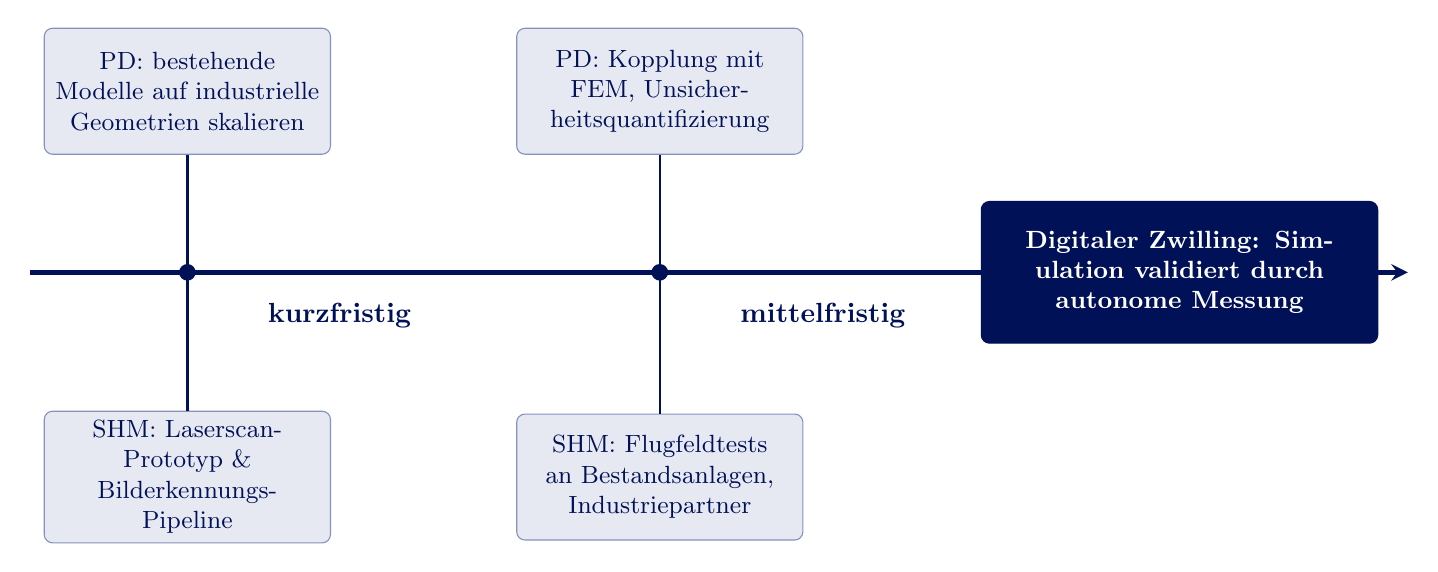
\begin{tikzpicture}[>=stealth, font=\normalsize]
  \draw[mainblue, line width=1.6pt, ->] (0,0) -- (17.5,0);
  \foreach \x/\lbl in {2/kurzfristig, 8/mittelfristig} {
    \fill[mainblue] (\x,0) circle (3pt);
    \node[mainblue, font=\bfseries, anchor=west] at (\x+0.9,-0.55) {\lbl};
  }
  \node[rectangle, rounded corners=3pt, draw=accent, fill=lightaccent, text=mainblue, text width=3.4cm, minimum height=1.6cm, font=\small, align=center] (b1) at (2,2.3) {PD: bestehende Modelle auf industrielle Geometrien skalieren};
  \node[rectangle, rounded corners=3pt, draw=accent, fill=lightaccent, text=mainblue, text width=3.4cm, minimum height=1.6cm, font=\small, align=center] (b2) at (2,-2.6) {SHM: Laserscan-Prototyp \& Bilderkennungs-Pipeline};

  \node[rectangle, rounded corners=3pt, draw=accent, fill=lightaccent, text=mainblue, text width=3.4cm, minimum height=1.6cm, font=\small, align=center] (b3) at (8,2.3) {PD: Kopplung mit FEM, Unsicherheitsquantifizierung};
  \node[rectangle, rounded corners=3pt, draw=accent, fill=lightaccent, text=mainblue, text width=3.4cm, minimum height=1.6cm, font=\small, align=center] (b4) at (8,-2.6) {SHM: Flugfeldtests an Bestandsanlagen, Industriepartner};

  \node[rectangle, rounded corners=3pt, draw=mainblue, fill=mainblue, text=white, text width=4.8cm, minimum height=1.8cm, font=\small\bfseries, align=center] (b5) at (14.6,0) {Digitaler Zwilling: Simulation validiert durch autonome Messung};

  \draw[mainblue, line width=0.9pt] (2,0) -- (b1.south);
  \draw[mainblue, line width=0.9pt] (2,0) -- (b2.north);
  \draw[mainblue, line width=0.9pt] (8,0) -- (b3.south);
  \draw[mainblue, line width=0.9pt] (8,0) -- (b4.north);
\end{tikzpicture}

\end{document}
